\documentclass[DD.tex]{subfiles}
\begin{document}

\section{Runtime view}
\subsection{Data acquisition Sequence Diagram}
\begin{figure}[h!]
\centering
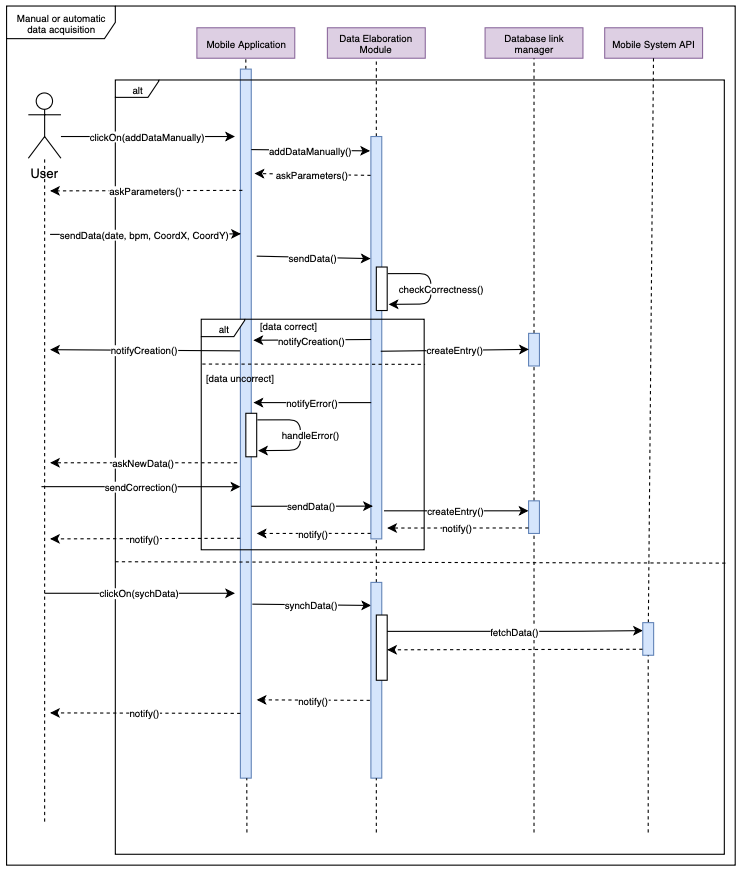
\includegraphics[height=16.00cm,keepaspectratio]{Figures/DataAcquisition}
\caption{Manual or automatic data acquisition sequence diagram}
\end{figure}



\subsection{AutomatedSOS Sequence Diagram}
\begin{figure}[h!]
\centering
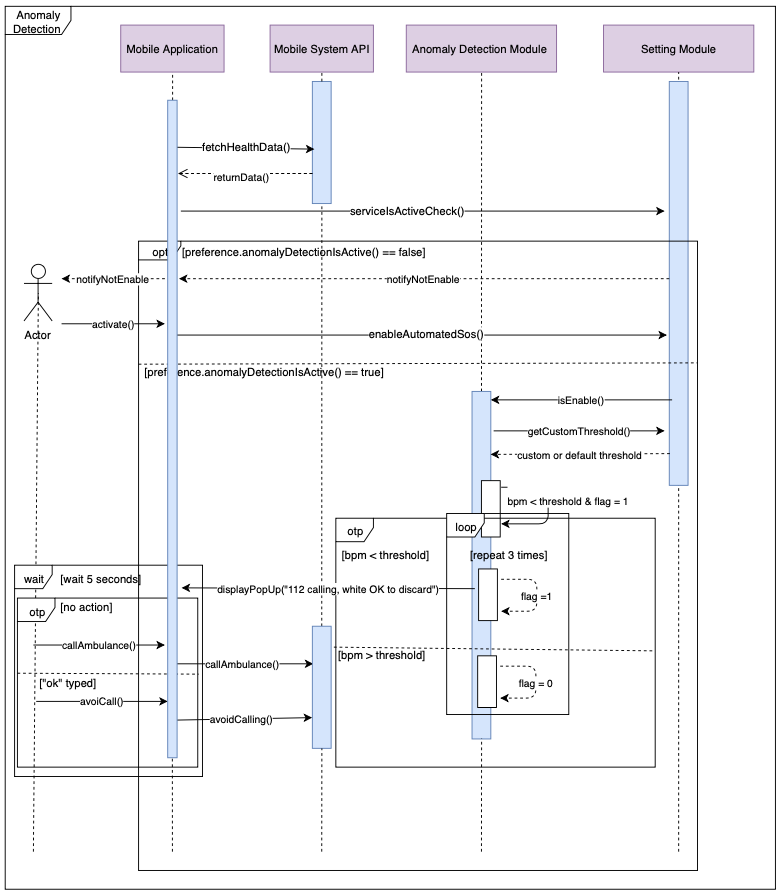
\includegraphics[height=17.00cm,keepaspectratio]{Figures/AutomatedSOS}
\caption{Automated SOS sequence diagram}
\end{figure}

The “\textbf{Anomaly Detection}” sequence diagram shown above represents the sequence of actions that may happen when an anomaly is detected.
The Mobile application, using the Mobile System’s API, fetches the data from the smartphone.
Whether the AutomatedSOS is enabled or disabled the behaviour of the platform is different.
The \textbf{Setting Module} is queried and if the Anomaly Detection is disable a notification is sent to the \textbf{Mobile App component} and the user will be able to activate the service or discard it.
Otherwise if it is enabled, the setting module is queried once again to obtain, if there exists, the custom threshold (otherwise the setting module component is going to return the default value).
Since now the \textbf{Anomaly Detection Module} check each bpm data received until it reads three values under the threshold, in this case it display on the user’s mobile application a \textbf{PopUp} with written “Warning! bpm under the minimum threshold”.
Now the user has 5 seconds to write “OK“ in the Text Field to discard the call.
\newpage


\subsection{Event Creation Sequence Diagram}
\begin{figure}[h!]
\centering
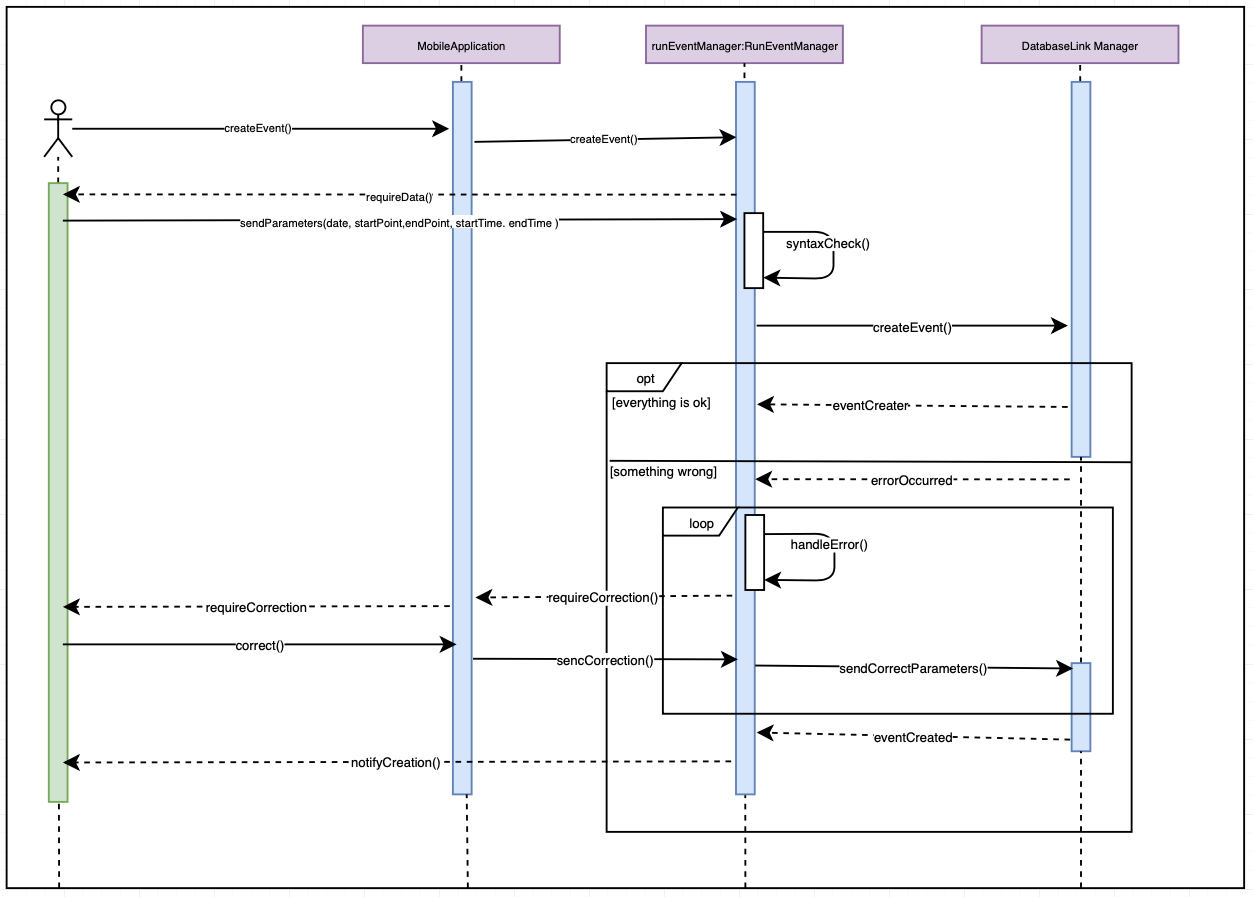
\includegraphics[height=10.00cm,keepaspectratio]{Figures/EventCreation}
\caption{Event creation sequence diagram}

The \textbf{Event Creation} Sequence Diagram shown above represents the sequence of actions that happen when a user tap on the button “create Event”.
When the application controller is triggered by the tap of the user sends to the \textbf{Run Event Manager} the request.
Since now the exchange is between the user and the component directly, in the sense that the control is entirely in the run event manager instead of in the mobile application component.
After that the data are collected by the manager, it sends a request of creation to the \textbf{Database Link Manager }that tries to perform the insertion
If everything goes correctly the event is created, otherwise the run event manager handle the error, and, if needed, it requires correction to the user directly.
At the end of the process the user is notified of the occurred event creation.
\end{figure}

\newpage

\end{document}